% !TEX root = ../../../main.tex
% 来源：中学数学实验教材·第二册（几何）
% 章节：直线形 / 面积与勾股定理
% 原始文件：3.tex，行 5166-5173
% 类型：tikz
% ---
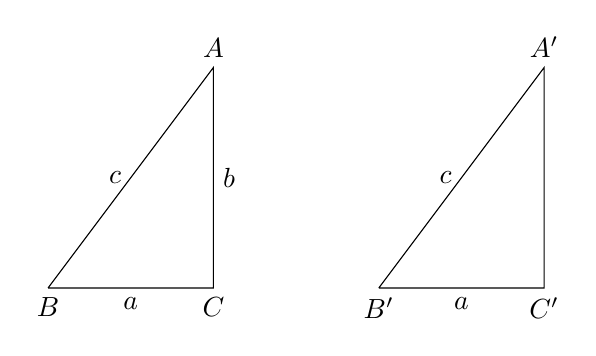
\begin{tikzpicture}[scale=.7]
\begin{scope}
\draw(0,0)node[below]{$B$}--node[below]{$a$}(3,0)node[below]{$C$}--node[right]{$b$}(3,4)node[above]{$A$}--node[left]{$c$}(0,0);
\end{scope}
\begin{scope}[xshift=6cm]
    \draw(0,0)node[below]{$B'$}--node[below]{$a$}(3,0)node[below]{$C'$}--(3,4)node[above]{$A'$}--node[left]{$c$}(0,0);
\end{scope}
\end{tikzpicture}
